\documentclass{report}
\usepackage{tikz}
\usepackage{listings, listings-rust}
\usepackage{titlesec}
\setcounter{secnumdepth}{4}
\usetikzlibrary{fit}
\usepackage[toc,section=section]{glossaries}

\tikzset{
    vertex/.style={
        circle,
        fill    = blue,
        outer sep = 2pt,
        inner sep = 1pt,
    }
}

%opening
\title{%
    EDB: Debugger for Ethereum's Programming Languages \\
	\medskip
	\large Report \#4: System Design \\
    \large Advised by Dr. Jackowitz	\\
	\large University of Scranton}
\author{Andrew Plaza}

\begin{document}
\maketitle
\newpage

\begin{abstract}
    \begin{enumerate}
        \item Hello
    \end{enumerate}
\end{abstract}

\tableofcontents
\newpage

\section{Introduction}
    The EDB client application may be launched via the shell with the `edb' command, which launches the main program routine for the binary. Depending upon the options the user has passed EDB, the main program will first connect to the locally-run ethereum test node the user has setup, which EDB references throughout the rest of its execution. The solidity source code file that will be debugged must also be provided by the user. From these inputs EDB creates two of it's highest-level abstractions, the File Model and the Emulator model, which make up the functionality of the debugger. The file model handles objects created by the compilation of the target source-language, such as the Abstract Syntax Tree, Source Mappings, and Bytecode. The Emulator model handles execution control and stores the Ethereum Virtual Machine(EVM) state at different steps in execution. State that is stored includes the current EVM Stack, Memory, and Non-Volatile Storage. Internally, the Emulator model uses the `sputnikvm' library. These parts make up the core of the debuggers functionality. Built on top of these items is also an optional JSON-RPC, which may be used in order to build featureful Graphical User Interfaces from 3rd-party applications.

    The design of EDB started first with a general development plan where models that were needed were identified. Based upon this plan, generic interfaces were created based upon the needs of the structure. Once this was complete, development was constrained to one part or sub-part of one model/interface, which worked towards fitting into the generic interface that was created during the first step. Unit tests were created alongside the original development of the part or sub-part, and testing took place to ensure the part worked individually before moving on to connect the part with the rest of the program. A kanban board on `Github Projects` was used in order to keep track of work that is under development, finished, or needs to be started.

\section{Levels}
\newpage
\subsection{High Level System Model}
\begin{center}
    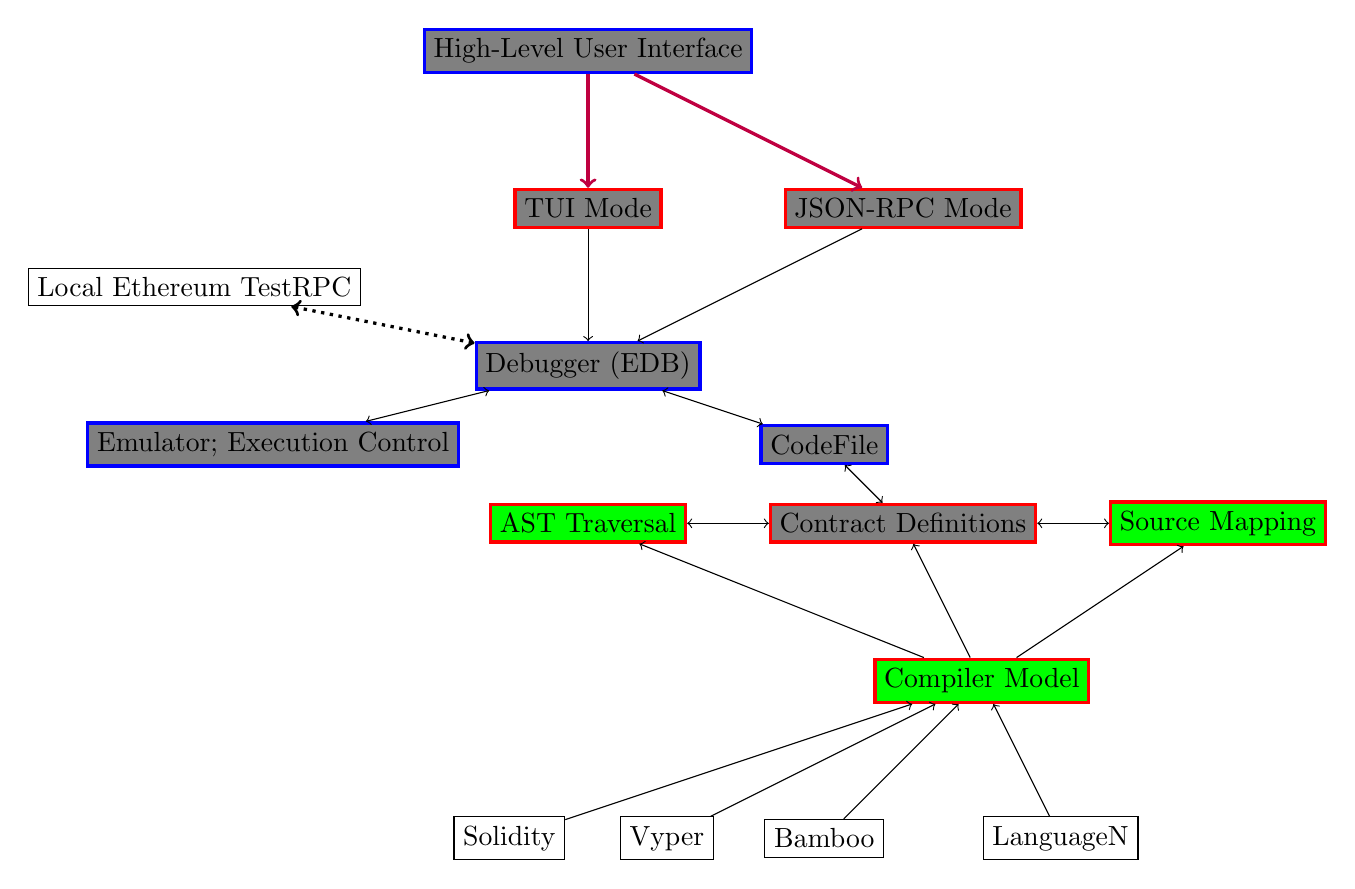
\begin{tikzpicture}

		\node[draw=blue,fill=gray,very thick] (CLI) at (8,10) {High-Level User Interface};

		\node[draw=red,fill=gray,very thick] (JSONRPC) at (12, 8) {JSON-RPC Mode};
		\node[draw=red,fill=gray,very thick] (TUIMode) at (8, 8) {TUI Mode};

		\node[draw] (ETH) at (3,7) {Local Ethereum TestRPC};

        \node[draw=blue,fill=gray,very thick] (EDB) at (8,6) {Debugger (EDB)};
        \node[draw=blue,fill=gray,very thick] (EVM) at (4, 5) {Emulator; Execution Control};
        \node[draw=blue,fill=gray,very thick] (CodeFile) at (11,5) {CodeFile};

        \node[draw=red,fill=green,very thick] (AST) at (8, 4) {AST Traversal};
        \node[draw=red,fill=gray,very thick] (Contracts) at (12, 4) {Contract Definitions};
        \node[draw=red,fill=green,very thick] (SrcMaps) at (16, 4) {Source Mapping};

        \node[draw=red,fill=green,very thick] (Compiler) at (13, 2) {Compiler Model};
        \node[draw] (Solidity) at (7, 0) {Solidity};
        \node[draw] (Vyper) at (9, 0) {Vyper};
        \node[draw] (Bamboo) at (11, 0) {Bamboo};
        \node[draw] (LanguageN) at (14,0) {LanguageN};

		\draw[->,draw=purple,very thick] (CLI) to (JSONRPC);
		\draw[->,draw=purple,very thick] (CLI) to (TUIMode);

		\draw[->,draw=black] (JSONRPC) to (EDB);
		\draw[->,draw=black] (TUIMode) to (EDB);


        \draw[<->,draw=black] (EDB) to (EVM);
        \draw[<->,draw=black] (EDB) to (CodeFile);
		\draw[<->,draw=black,dotted,very thick] (EDB) to (ETH);

        \draw[<->,draw=black] (Contracts) to (AST);
        \draw[<->,draw=black] (Contracts) to (SrcMaps);
        \draw[<->,draw=black] (CodeFile) to (Contracts);

        \draw[<-,draw=black] (AST) to (Compiler);
        \draw[<-,draw=black] (SrcMaps) to (Compiler);
        \draw[<-,draw=black] (Contracts) to (Compiler);

        \draw[->,draw=black] (Solidity) to (Compiler);
        \draw[->,draw=black] (Vyper) to (Compiler);
        \draw[->,draw=black] (Bamboo) to (Compiler);
        \draw[->,draw=black] (LanguageN) to (Compiler);
        %%% Color Legend
	\end{tikzpicture}
\end{center}
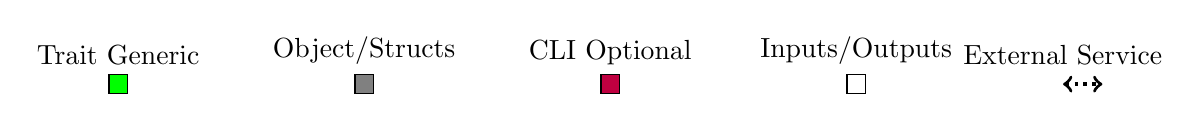
\begin{tikzpicture}
	\node [label=Trait Generic,draw,fill=green] (node1) {};
	\node [label={[name=l] Object/Structs},draw,fill=gray] (node2) at ([xshift=3cm]node1.east){};
	\node [label={[name=l] CLI Optional},draw,fill=purple] (node3) at ([xshift=3cm]node2.east){};
    \node [label={[name=l] Inputs/Outputs},draw] (node4) at ([xshift=3cm]node3.east){};
    \node [label={[name=l] External Service}] (node5) at ([xshift=2.5cm]node4.east){};
	\draw [<->,draw=black,dotted,very thick] (12,0) to (12.5,0);
\end{tikzpicture}
\vspace*{1cm}

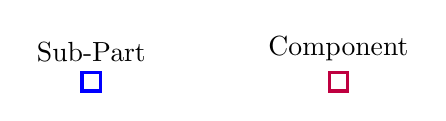
\begin{tikzpicture}
    \node [label=Sub-Part,draw=blue,very thick] (node1) {};
    \node [label={[name=l] Component},draw=purple, very thick] (node2) at ([xshift=3cm]node1.east){};
\end{tikzpicture}

\newpage

\subsection{User Interface Modes}
    \subsubsection{Abstract Specification}
    \subsubsection{Algorithm Design}
    \subsubsection{Component: TUI Mode}
    \subsubsection{Component: JSON-RPC Mode}


\subsection{Debugger Core, EDB}
    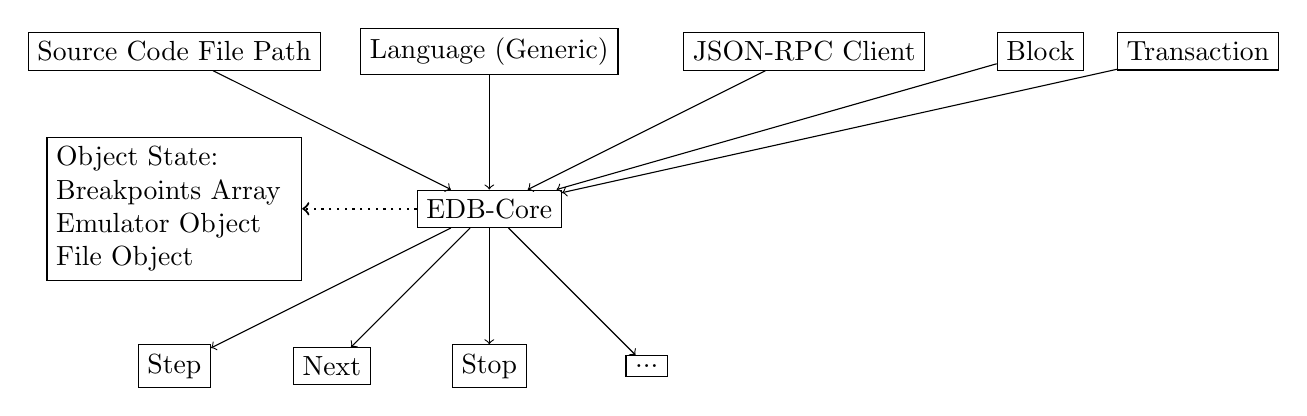
\begin{tikzpicture}
        \node[draw] (File) at (0,4) {Source Code File Path};
        \node[draw] (Language) at (4,4) {Language (Generic)};
        \node[draw] (Client) at (8,4) {JSON-RPC Client};
        \node[draw] (Block) at (11,4) {Block};
        \node[draw] (Transaction) at (13,4) {Transaction};


        \node[draw] (EDB-Core) at (4,2) {EDB-Core};

        \node[draw,text width=3cm] (Object State) at (0, 2) {Object State:\
            Breakpoints Array\
            Emulator Object\
            File Object};

        \node[draw] (Step) at (0,0) {Step};
        \node[draw] (Next) at (2,0) {Next};
        \node[draw] (Stop) at (4,0) {Stop};
        \node[draw] (etc) at (6,0) { ... };

        \draw[->,draw,dotted,thick] (EDB-Core) to (Object State);
        \draw[->,draw] (Language) to (EDB-Core);
        \draw[->,draw] (Client) to (EDB-Core);
        \draw[->,draw] (Block) to (EDB-Core);
        \draw[->,draw] (Transaction) to (EDB-Core);
        \draw[->,draw] (EDB-Core) to (Step);
        \draw[->,draw] (EDB-Core) to (Next);
        \draw[->,draw] (EDB-Core) to (Stop);
        \draw[->,draw] (EDB-Core) to (etc);
        \draw[->,draw] (File) to (EDB-Core);
    \end{tikzpicture}


    \subsubsection{Abstract Specification}
        The Debugger core provides all the core debugging features one may expect a debugger to offer. This level is not concerned with parsing input or events that the user may trigger. Instead, it works with input that has already been parsed. Namely, the Ethereum Language Trait, a JSON-RPC Client, and parameters for the transaction the user wishes to debug. Sourcemapping and EVM Execution control is done implicitly through the debug functions: 'step', 'next', 'stop', 'restart', etc. Therefore, this level mostly serves as a higher-level abstraction over the next two levels 'Emulator' and 'CodeFile'. This level accepts the source code file, a object which implements the trait 'Language', a JSON-RPC client to communicate with the locally running Ethereum Test Node, along with the block and transaction the user wishes to debug. From these inputs, creation of the Emulation and Source Mapping objects is enabled.

    \subsubsection{Interface Design}
        This level should be able to provide all the debug functions needed in order to debug a source code file. It should not expose any objects or functions which deal with Source Mapping or Ethereum Virtual Machine emulation. It is assumed that inputs provided to this interface match up with information that is present in the local test ethereum node. Necessarily this indicates that the compiled bytecode of the source code provided matches with bytecode that has already been deployed onto the Ethereum Test Node. This level should provide a programmatic view of the functions outlined in the requirements specification, namely:
    \begin{itemize}
        \item \textbf{step}: step forward to the next source-line in execution
        \item \textbf{stepback}: step back one source-line in execution
        \item \textbf{print}: print stack, memory, or variables in the program
        \item \textbf{printline}: print the current line in the source code that execution is at
        % \item \textbf{printlines}: print a number of lines relative to the current line code execution is at in source code
        %\item \textbf{set_breakpoint}: set a breakpoint at a line number in the source code where execution will stop
        %\item \textbf{unset_breakpoint}: Unset a breakpoint at a line number
        \item \textbf{restart}: restart execution entirely from a clean Ethereum Virtual Machine state
        \item \textbf{run}: run a function in the source code (accepts arguments according to function parameters)
        \item \textbf{next}: Continue execution to the next breakpoint
        \item \textbf{previous}: Take execution back to the previous breakpoint
        \item \textbf{stepinto}: Step into a function (if the current line contains a function call)
    \end{itemize}

    \subsubsection{Component: Address Cache}
    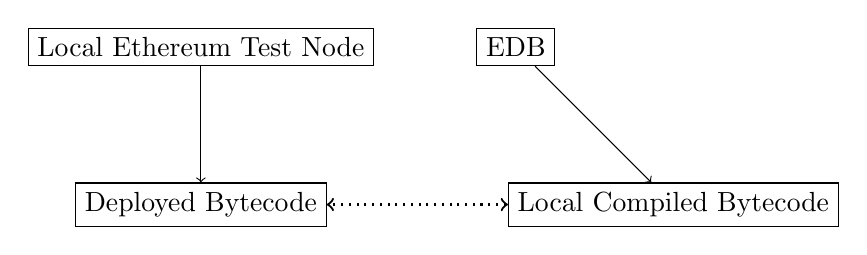
\begin{tikzpicture}
        \node[draw] (TestNode) at (0, 4) {Local Ethereum Test Node};
        \node[draw] (DeployedBytecode) at (0, 2) {Deployed Bytecode};
        \node[draw] (EDB) at (4, 4) {EDB};
        \node[draw] (LocalBytecode) at (6, 2) { Local Compiled Bytecode};

        \draw[->,draw] (TestNode) to (DeployedBytecode);
        \draw[->,draw] (EDB) to (LocalBytecode);
        \draw[<->,draw,dotted,thick] (LocalBytecode) to (DeployedBytecode);
    \end{tikzpicture}

        In order to associate information provided by the user in the form of a source code file, a component to match up the compiled bytecode created from the file provided by the user to an address existing in the Ethereum Test Node is necessary. This information is needed throughout transaction execution in case the Ethereum Virtual Machine is in need of any state existing on the blockchain before execution has started. Therefore, a local cache of all known addresses and associated compiled bytecode is created once the debugger is first launched. This cache is stored as a HashMap: The key is a 160bit address (The Address of the Ethereum Account owning the code) and the value is the compiled bytecode. This information is gathered and updated whenever the EDB client is run by crawling all addresses known to the local Ethereum node. It is up to the user whether to refresh this information on each run of the debugger, therefore not storing any persistant state on-disk, or to write this cache to be retrieved on the next run of the debugger. Since only one contract is being debugged at a time, the address cache is only queried once for the relevant address and bytecode. The cache object is not stored along with the Object State, since later retrieval may be done via the filesystem if requested by the user.

    \subsubsection{Component: Breakpoints}
        Breakpoints are set and unset by two functions 'set\_breakpoint' and 'unset\_breakpoint'. These are stored in a simple array. Each breakpoint serves as an indicator as to where execution should stop for the rest of the debug functions. For instance, in order to begin debugging the `set\_breakpoint' function of the EDB interface is called first. Once `run' is called after that, execution is expected to continue up to and only until that line in the original source code file. Each consequent `step' call is expected to run only until the next line in the source code, while a `next' call would be expected to run to the next breakpoint.

\subsection{Emulator, Execution Control}
    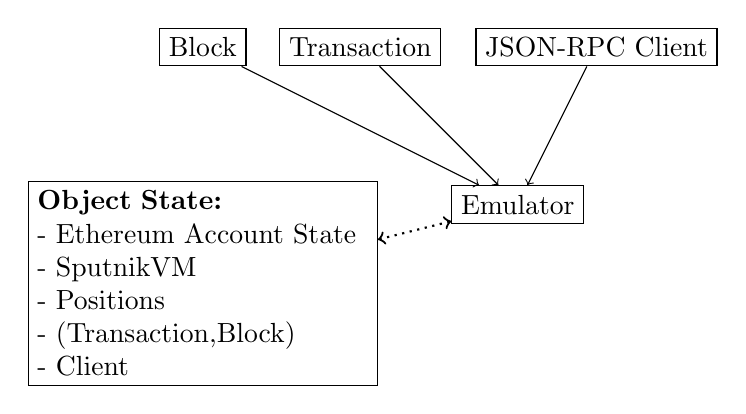
\begin{tikzpicture}
        \node[draw] (Block) at (0, 4) {Block};
        \node[draw] (Transaction) at (2, 4) {Transaction};
        \node[draw] (Client) at (5,4) {JSON-RPC Client};
         \node[draw] (Emulator) at (4, 2) { Emulator };

        \node[draw,text width=4.2cm] (Object State) at (0, 1) {\textbf{Object State:}\\
                - Ethereum Account State\\
                - SputnikVM\\
                - Positions\\
                - (Transaction,Block)\\
                - Client\\};
        \draw[->,draw] (Block) to (Emulator);
        \draw[->,draw] (Transaction) to (Emulator);
        \draw[->,draw] (Client) to (Emulator);
        \draw[<->,draw,dotted,thick] (Emulator) to (Object State);

    \end{tikzpicture}

    \subsubsection{Abstract Specification}
        The Emulator provides execution control for the debugger level. This means it deals at the Opcode and Instruction level, stores and exposes state related to the Ethereum Virtual Machine, and handles any blockchain state requirements it may need from the local ethereum test node. The 'Transaction' and 'Block' inputs mostly contain extraneous information that is unnecessary to debugging but necessary to general Ethereum Transaction Execution, except for the bytecode which is apart of the 'Transaction' input object. The Emulator, however, is not concerned with lines in the source code, breakpoints, or any 'human-decipherable' meaning which may be attached to items that reside in the Ethereum Virtual Machine state. It is able to decipher individual opcodes from Instructions, as well as identify how those opcodes contribute to the next state of the Ethereum Virtual Machine. At it's lowest level, an Ethereum Virtual Machine library, `sputnikvm` is used in order to carry out these instructions and general code execution. In addition, the Emulator keeps the Stack, Memory, and Non-Volatile storage in sync with the local ethereum test node, and is able to access these data-structures at-will (without any constraints).

    \subsubsection{Interface Design}
        The interface of the Debugger and Emulator level hold many similiarites. For instance, the Emulator is able to `step\_forward`, `step\_back`, and `run\_until` a certain point in execution has been reached. However, instead of stepping over lines in source code, functions at the Emulator level deal only with stepping instructions in the bytecode. Therefore, 'step\_forward' means execute the next instruction in the bytecode array, and 'step\_back' means to step back to the overall state before the current instruction had been executed. Functions to peek at the current state of the Virtual Machine are also exposed, in order to faciliate variable-decoding at in the Debugger level.

    \subsubsection{Algorithm Design}
    \subsubsection{Data Strucure Design}
    \subsubsection{Component: Persistant Account State}
    \subsubsection{Component: Opcode and Instruction Mappings}

\subsection{CodeFile}
    \subsubsection{Abstract Specification}
    \subsubsection{Interface Design}
    \subsubsection{Component: Contract File}
    \subsubsection{Component: Contract}
    \subsubsection{Component: AST Traversal}
    \subsubsection{Component: Source Mapping}
    \subsubsection{Component: Compiler}
    \subsubsection{Component: Variable Decoding}

\section{User Interface}

-- What To Do:
    - Provide a 'Abstract Spec' of every component (Debugger, Compilier, Source Map, AST, Contracts, CodeFile, etc)
        - provide data structs, and component design of every piece of that (graph it out. Graphs don't have to be as complicated as first. But enough to get the gist of the design of the compnonent)
        -

Test Rust Code
\begin{lstlisting}[language=Rust]
    pub trait Foo {
        fn killAllBunnies<F>(fun: F) -> AstItem
        where
            F: Fn(&mut AbstractFunction) -> bool;
        fn scrapeWebForSkynet();
    }
\end{lstlisting}
\section{Help System}

\section{}

\end{document}
